%!TEX root = ../thesis.tex
\chapter{Robust Deep Learning System for Multi-Sensor Road Detection}
\label{ch:app1}

\ifpdf
\graphicspath{{Appendix1/Figs/Raster/}{Appendix1/Figs/PDF/}{Appendix1/Figs/}}
\else
\graphicspath{{Appendix1/Figs/Vector/}{Appendix1/Figs/}}
\fi

Applications of machine learning algorithms have become commonplace in automotive research, particularly the use of techniques such as deep neural networks for complex image processing tasks including object identification and tracking. In this article we describe a hardware accelerated, end-to-end deep learning solution for the most fundamental driving safety task; road keeping. We use an Autonomous Formula-SAE vehicle equipped with multiple LiDARs, high resolution camera and NVIDIA Jetson TX1 compute platform. We examine the issues surrounding reliability of such an algorithm and how this is mitigated by using an array of sensors to provide redundancy of raw information, as well as presenting a training and testing methodology

\section{Introduction}
The Renewable Energy Vehicle Project (REV) operates a compact Formula SAE race car as a platform for hardware-in-the-loop solution development (see Fig.~\ref{fig:a:car}). The system features a modular software structure utilising Robot Operating System (ROS) to maintain functions of perception, path planning, mapping and control and is practicable for driving in structured and unstructured driving environments.

Recently, autonomous driving is a topic of much interest in the public domain, with commercial vehicles accessible to the public expected at the beginning of the next decade~\cite{bimbraw_autonomous_2015}. The technological advances in communications, controls and embedded systems have created an environment conducive with the implementation of fully autonomous solutions, however, one of the main barriers to the adoption of autonomous cars on the roads is public trust~\cite{kaur_trust_2018}. Research into driverless technology should address the factors of performance expectancy, reliability and security as they are now the key factors influencing driverless car adoption~\cite{kaur_trust_2018}. 

The priority of road detection is to ensure safe driving and has been commonly implemented using LiDAR or cameras. A key outcome in recent applications is the shift toward the use of sensor fusion to obtain a larger dataset. LiDAR is effective at detecting objects and generating an accurate hypothesis for their position, while vision is used as a classifier responsible for validation or final classification of objects. The result of combining LiDAR and camera data prior to processing has provided improvements in the false positive rate~\cite{han_road_2017}. An end-to-end or sensor-to-control implementation utilising machine learning will introduce efficiencies in the processing of data via a Deep Neural Network~\cite{bojarski_end_2016}.

\begin{figure}[ht] 
	\centering    
	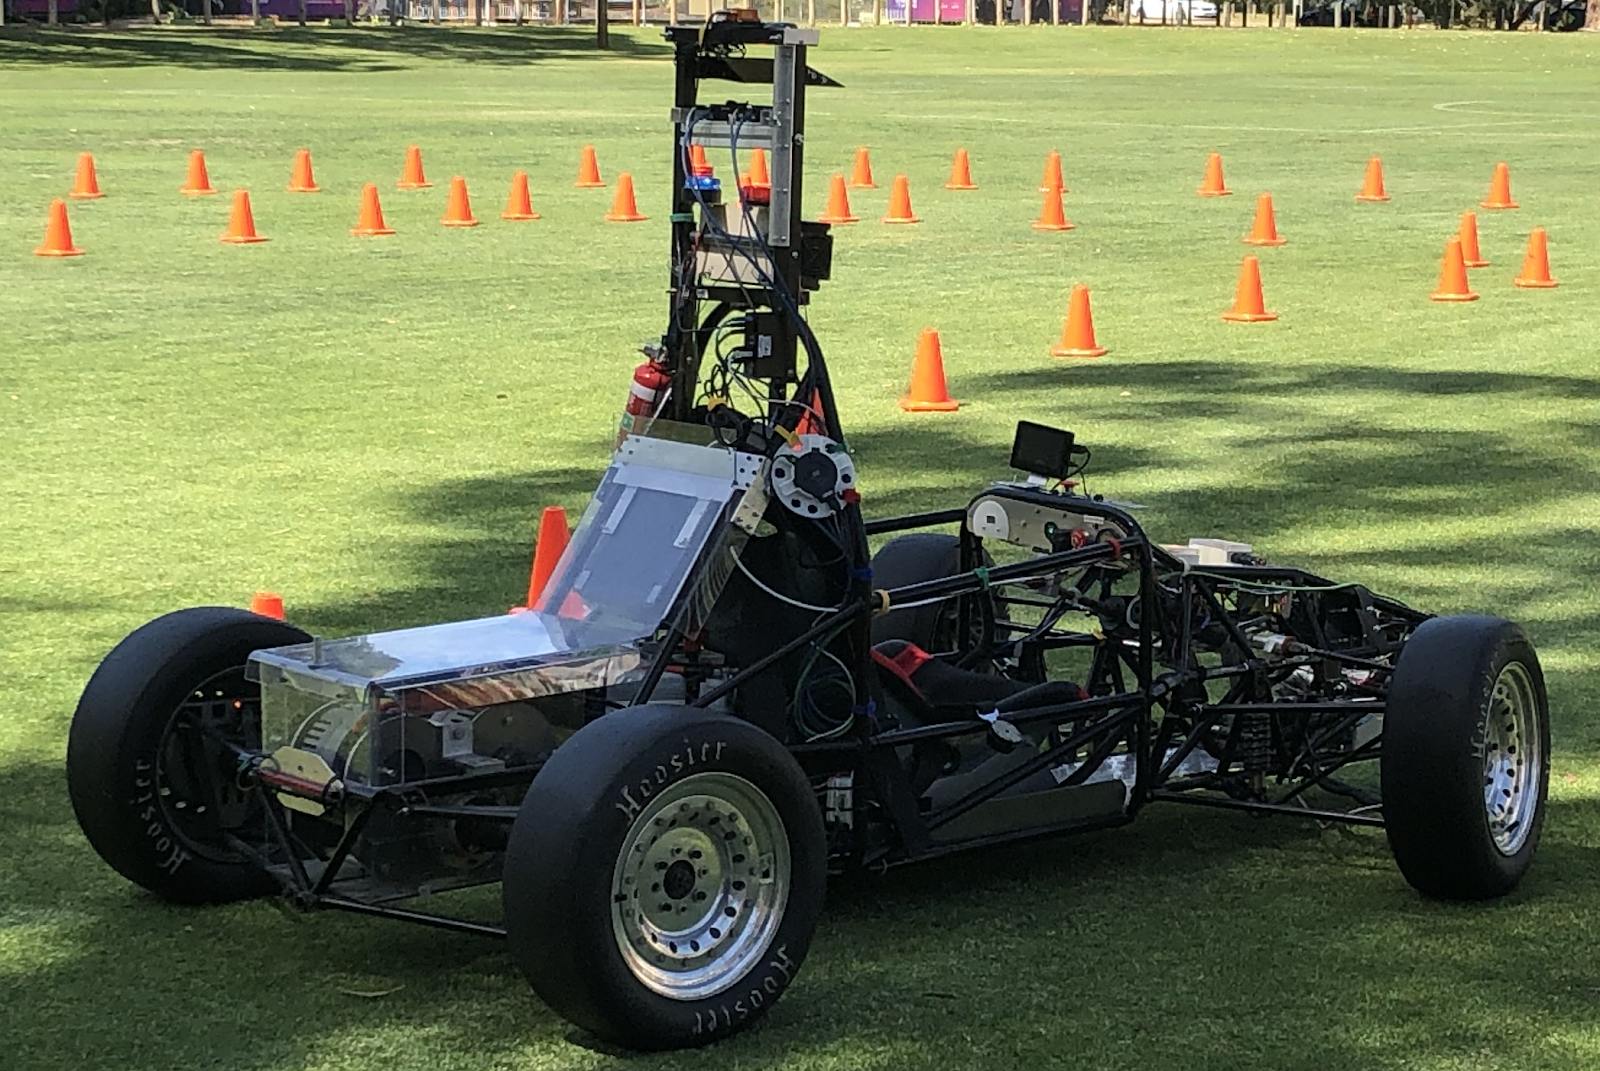
\includegraphics[width=0.7\textwidth]{car}
	\caption{UWA-REV Autonomous SAE-Electric car.}
	\label{fig:a:car}
\end{figure}

\section{Problem Description}
Road detection is a vital pillar in autonomous driving and care must be taken to ensure a robust approach for all autonomous applications in order to maintain public expectations. The single sensor based approaches previously adopted does not utilise the data to its full extent and is inferior to an approach where sensor fusion is applied~\cite{han_road_2017}. LiDAR is not strongly affected by environmental conditions while vision based methods suffer greatly from variations in light intensity and limited fields of view, but can provide greater performance through identification of a larger feature space. The multisensory approach is capable of utilising the strengths of each sensor, improving the overall robustness.

\section{Sensor Configuration}
The Formula-SAE car features an array of sensors, including two cameras, three LiDARs, a high-performance inertial navigation system as well as odometry and GPS. For road keeping, we focus on using environmental sensing to provide redundancy in case of inaccurate localisation.

\subsection{Computer Vision}
A pair of FLIR Blackfly GigE cameras are mounted on the vehicle’s frame to perform tasks related to visual navigation, such as semantic segmentation and visual odometry.  These cameras are fitted with wide-aperture varifocal lenses and use 1.3MP 1/3" global shutter CCD image sensors. The cameras are connected via Gigabit Ethernet to the Jetson TX1, interfacing them through Blackfly’s ROS node where it is configured to record at 10 Hz per channel.

\subsection{LiDAR}
The vehicle utilises an array of Light Distance and Ranging (LiDAR) systems. This consists of a SICK LMS111-1010, an ibeo LUX 4, and a Velodyne VLP-16 connected via Ethernet to the NVIDIA Jetson TX1. The data is published by each of the LiDARs’ ROS drivers and made available for processing within ROS. 

The LMS111 is mounted forward-facing on the front of the vehicle and scans a single layer at 50 Hz. The LUX scans four layers at 10 Hz and features in-built object detection and tracking. It is utilised to achieve road edge and object detection at a distance. The VLP-16 scans 16 layers at 20 Hz, and is mounted in the horizontal plane at the top of the vehicle, resulting in scans of the ground at distances from 5 to 45 metres ahead of the vehicle and can be used for LiDAR-based mapping tasks.

\section{Proposed Pipeline and Algorithms}
Our approach uses a hybrid of three components, combining traditional engineering approaches with deep learning methods, to achieve a more efficient and robust system.

\subsection{LiDAR Road Edge Detection}
Road edge-detection with LIDAR can be accomplished by means of either locating the road-body itself, or by location of an edge feature. Currently, both approaches have been tested using novel algorithms such as~\cite{t._drage_integration_2014}. The nature of the data lends itself well to processing by CNN which, with sufficient training, will be sensitive to both detection conditions.

\subsection{Semantic Image Segmentation}
We use semantic segmentation to understand and account for the large dynamism in road scenes, such as moving pedestrians and traffic, as well as variations in road types and markings. Semantic segmentation uses a convolutional neural network (CNN) to classify each pixel on an image frame to constitute an object that it represents. It outputs a series of image, each composed from a set of several distinct colours, with each colour representing an object class. To cater for the dynamism of road environments, we further classify these objects into static and dynamic objects. Through the segregation of static and dynamic objects, the system can then direct and curate computation methods for different regions within an image frame. For instance, calculations on the road region with lane markers will yield results pertaining to lane keeping, centring the vehicle as it drives. 

\subsection{End-to-End Deep Learning}
We describe an end-to-end CNN architecture which differs from~\cite{bojarski_end_2016} in that it processes the camera input image ($50\times200$ greyscale pixels) in a separate stack from the combined LiDAR input scan ($50\times200$ distance values). Each side runs several convolutional $5\times5$ kernel layers until both streams get linked together with convolutional and fully connected layers. A final output layer of five neurons defines the desired steering angle through linear interpolation. This architecture is illustrated as Fig.~\ref{fig:a:network}.

In this application we propose an end-to-end solution which accepts both image data and LIDAR point clouds as input to a deep CNN and generates driving command directly. Training data is being collected using the sensor array on the SAE car itself. Depth information provided by different LiDARs is then merged into a 3D point clouds. Then by projecting the point clouds to the surrounding cylindrical plane of the vehicle, the data can be presented as a 2D array, which can be processed computationally efficiently by CNN. The training data is developed with sensor failures and typical anomalies for each sensor integrated into the training set such that the model is robust under failure of each sensor. The controller output is then used for lane-keeping via the ROS controller node.

\begin{figure}[ht] 
	\centering    
	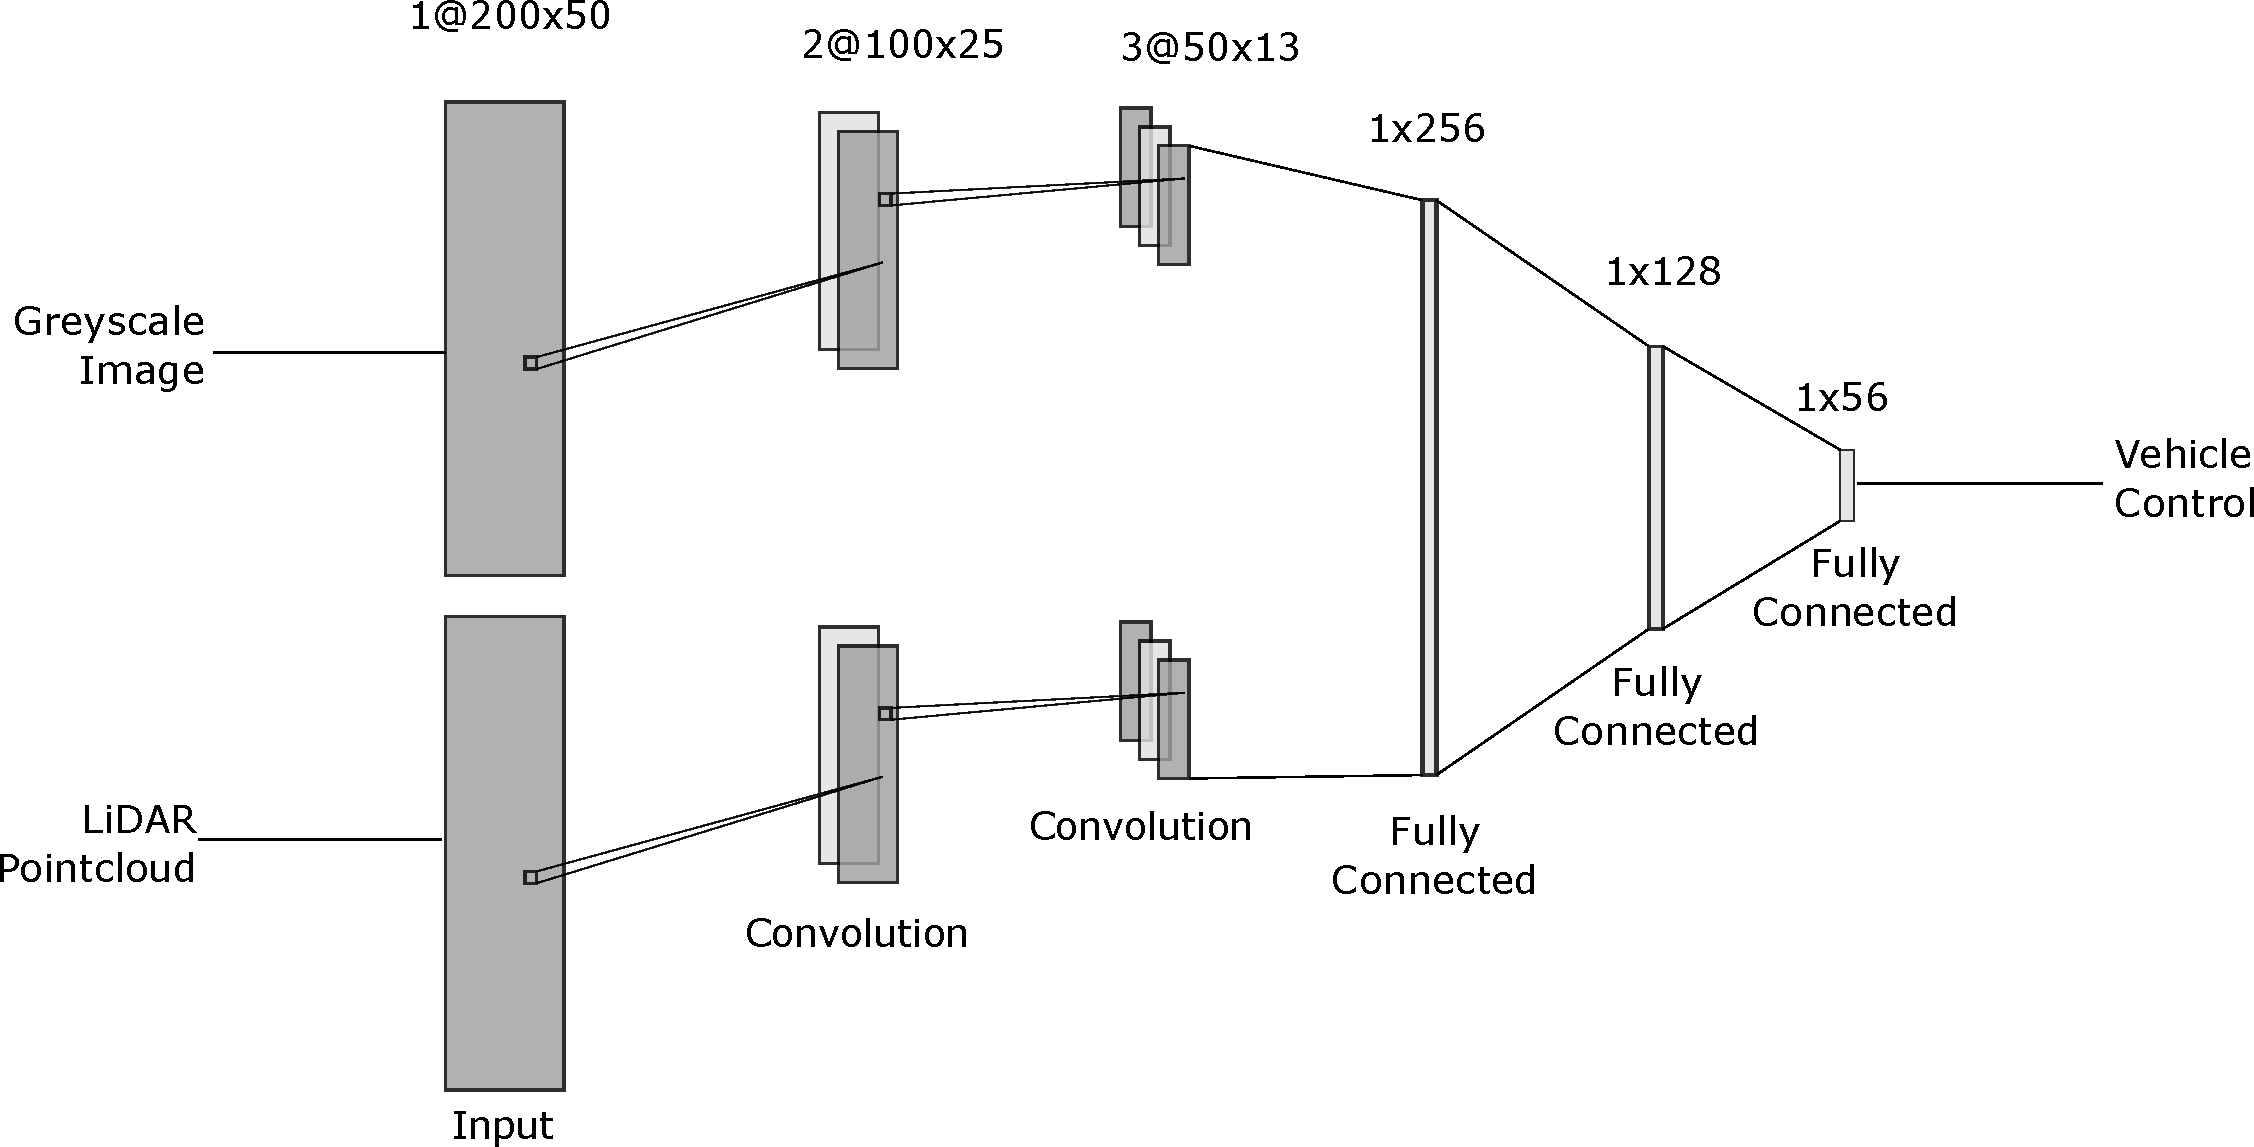
\includegraphics[width=\textwidth]{network}
	\caption{Hybrid CNN architecture for camera and LiDAR.}
	\label{fig:a:network}
\end{figure}

\subsection{Simulation Framework and Experiments}
A hardware-in-the-loop autonomous driving simulation platform centred around the CARLA driving simulator is utilised for both the collection of training data, and early stage testing of the developed algorithms. The use of simulation in the establishment of a training data set allows for improved efficiency in the case of semantic segmentation, with the capability to automatically generate pixel-perfect segmentation masks. It also allows the training set to include a broader range of scenarios than are available to the real hardware platform. 

We augment simulation with field testing on roads and poorly defined paths, to prove the performance under varied conditions. The robustness of this approach is proven by demonstration that the redundancy of multiple sensors leads to a fault tolerance and high accuracy suitable to ensure trustworthy road-keeping.


%% ******************************* Thesis Appendix A ****************************
%\chapter{How to install \LaTeX} 
%
%\section*{Windows OS}
%
%\subsection*{TeXLive package - full version}
%\begin{enumerate}
%\item	Download the TeXLive ISO (2.2GB) from\\
%\href{https://www.tug.org/texlive/}{https://www.tug.org/texlive/}
%\item	Download WinCDEmu (if you don't have a virtual drive) from \\
%\href{http://wincdemu.sysprogs.org/download/}
%{http://wincdemu.sysprogs.org/download/}
%\item	To install Windows CD Emulator follow the instructions at\\
%\href{http://wincdemu.sysprogs.org/tutorials/install/}
%{http://wincdemu.sysprogs.org/tutorials/install/}
%\item	Right click the iso and mount it using the WinCDEmu as shown in \\
%\href{http://wincdemu.sysprogs.org/tutorials/mount/}{
%http://wincdemu.sysprogs.org/tutorials/mount/}
%\item	Open your virtual drive and run setup.pl
%\end{enumerate}
%
%or
%
%\subsection*{Basic MikTeX - \TeX~ distribution}
%\begin{enumerate}
%\item	Download Basic-MiK\TeX (32bit or 64bit) from\\
%\href{http://miktex.org/download}{http://miktex.org/download}
%\item	Run the installer 
%\item	To add a new package go to Start >> All Programs >> MikTex >> Maintenance (Admin) and choose Package Manager
%\item	Select or search for packages to install
%\end{enumerate}
%
%\subsection*{TexStudio - \TeX~ editor}
%\begin{enumerate}
%\item	Download TexStudio from\\
%\href{http://texstudio.sourceforge.net/\#downloads}
%{http://texstudio.sourceforge.net/\#downloads} 
%\item	Run the installer
%\end{enumerate}
%
%\section*{Mac OS X}
%\subsection*{MacTeX - \TeX~ distribution}
%\begin{enumerate}
%\item	Download the file from\\
%\href{https://www.tug.org/mactex/}{https://www.tug.org/mactex/}
%\item	Extract and double click to run the installer. It does the entire configuration, sit back and relax.
%\end{enumerate}
%
%\subsection*{TexStudio - \TeX~ editor}
%\begin{enumerate}
%\item	Download TexStudio from\\
%\href{http://texstudio.sourceforge.net/\#downloads}
%{http://texstudio.sourceforge.net/\#downloads} 
%\item	Extract and Start
%\end{enumerate}
%
%
%\section*{Unix/Linux}
%\subsection*{TeXLive - \TeX~ distribution}
%\subsubsection*{Getting the distribution:}
%\begin{enumerate}
%\item	TexLive can be downloaded from\\
%\href{http://www.tug.org/texlive/acquire-netinstall.html}
%{http://www.tug.org/texlive/acquire-netinstall.html}.
%\item	TexLive is provided by most operating system you can use (rpm,apt-get or yum) to get TexLive distributions
%\end{enumerate}
%
%\subsubsection*{Installation}
%\begin{enumerate}
%\item	Mount the ISO file in the mnt directory
%\begin{verbatim}
%mount -t iso9660 -o ro,loop,noauto /your/texlive####.iso /mnt
%\end{verbatim}
%
%\item	Install wget on your OS (use rpm, apt-get or yum install)
%\item	Run the installer script install-tl.
%\begin{verbatim}
%	cd /your/download/directory
%	./install-tl
%\end{verbatim}
%\item	Enter command `i' for installation
%
%\item	Post-Installation configuration:\\
%\href{http://www.tug.org/texlive/doc/texlive-en/texlive-en.html\#x1-320003.4.1}
%{http://www.tug.org/texlive/doc/texlive-en/texlive-en.html\#x1-320003.4.1} 
%\item	Set the path for the directory of TexLive binaries in your .bashrc file
%\end{enumerate}
%
%\subsubsection*{For 32bit OS}
%For Bourne-compatible shells such as bash, and using Intel x86 GNU/Linux and a default directory setup as an example, the file to edit might be \begin{verbatim}
%edit $~/.bashrc file and add following lines
%PATH=/usr/local/texlive/2011/bin/i386-linux:$PATH; 
%export PATH 
%MANPATH=/usr/local/texlive/2011/texmf/doc/man:$MANPATH;
%export MANPATH 
%INFOPATH=/usr/local/texlive/2011/texmf/doc/info:$INFOPATH;
%export INFOPATH
%\end{verbatim}
%\subsubsection*{For 64bit OS}
%\begin{verbatim}
%edit $~/.bashrc file and add following lines
%PATH=/usr/local/texlive/2011/bin/x86_64-linux:$PATH;
%export PATH 
%MANPATH=/usr/local/texlive/2011/texmf/doc/man:$MANPATH;
%export MANPATH 
%INFOPATH=/usr/local/texlive/2011/texmf/doc/info:$INFOPATH;
%export INFOPATH
%
%\end{verbatim}
%
%
%
%%\subsection{Installing directly using Linux packages} 
%\subsubsection*{Fedora/RedHat/CentOS:}
%\begin{verbatim} 
%sudo yum install texlive 
%sudo yum install psutils 
%\end{verbatim}
%
%
%\subsubsection*{SUSE:}
%\begin{verbatim}
%sudo zypper install texlive
%\end{verbatim}
%
%
%\subsubsection*{Debian/Ubuntu:}
%\begin{verbatim} 
%sudo apt-get install texlive texlive-latex-extra 
%sudo apt-get install psutils
%\end{verbatim}
